\documentclass[11pt]{article}
\usepackage[margin=1in]{geometry}
\usepackage{amsmath,amssymb,amsthm,mathtools}
\usepackage{graphicx}
\usepackage{microtype}
\usepackage[hidelinks]{hyperref}

\newtheorem{theorem}{Theorem}
\newtheorem{lemma}{Lemma}
\newcommand{\R}{\mathbb R}
\newcommand{\N}{\mathbb N}

\title{Removing Reflexivity Alone Does Not Preserve\\
Hammerstein Solvability}
\author{Automated mathematics run \texttt{fa\_banach\_001}, lane 7}
\date{August 11, 2026}

\begin{document}
\maketitle

\begin{center}
\fbox{\parbox{0.9\textwidth}{\textbf{Status.}
Candidate full counterexample, likely valid, pending expert review.
The Hammerstein existence hypotheses (4.2)--(4.6) of
Barroso--O'Regan do not remain sufficient when reflexivity is simply deleted.
Failure occurs on real $\ell_1$ with a constant kernel and a bounded globally
Lipschitz nonlinearity, even when the growth ratio in (4.6) is zero.}}
\end{center}

\section{Source question and precise answer}

Barroso and O'Regan consider
\begin{equation}\label{eq:hammerstein}
 y(t)=h(t)+\int_0^1 k(t,s)f(s,y(s))\,ds,
 \qquad 0\leq t\leq1,
\end{equation}
where $f(s,\cdot)$ is weakly sequentially continuous, $h$ is continuous,
$k(t,\cdot)\in L^1$, and $t\mapsto k(t,\cdot)$ is $L^1$-continuous.  Their
growth assumptions are
\[
 \|f(s,x)\|\leq\Omega(\|x\|),\qquad
 K\limsup_{r\to\infty}\frac{\Omega(r)}r\leq1,
 \quad K=\sup_t\int_0^1|k(t,s)|\,ds.                 \tag{4.5--4.6}
\]
They explain that the known proof for reflexive $E$ uses weak compactness and
ask what conditions are needed if reflexivity is removed~\cite[pp.~6--7]{source}.

\begin{figure}[ht]
  \centering
  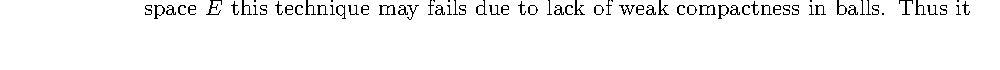
\includegraphics[width=0.94\textwidth]{figures/question_lead_crop.png}
  \vspace{2mm}
  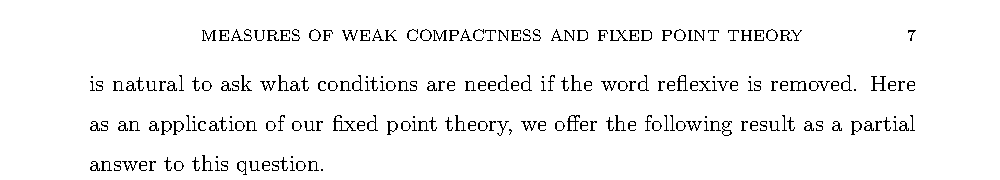
\includegraphics[width=0.94\textwidth]{figures/question_page7_crop.png}
  \caption{The question as printed across the bottom of page 6 and the top of
  page 7 of arXiv:math/0310422.  Conditions (4.5)--(4.6) are transcribed above.}
  \label{fig:question}
\end{figure}

The question is open-ended.  We settle its strongest natural yes/no
interpretation negatively: conditions (4.2)--(4.6) alone do \emph{not} imply
solvability in an arbitrary Banach space.  Some genuine replacement for
reflexive weak compactness is necessary.

\subsection*{Proof intuition}

With the constant kernel $k\equiv1$ and $h=0$, the right side of
\eqref{eq:hammerstein} does not depend on $t$.  Every solution must therefore
be constant, and the integral equation collapses to a fixed-point equation
$c=F(c)$.  We build a bounded fixed-point-free map $F$ on $\ell_1$.  Normally,
norm continuity would not meet the required weak sequential continuity, but
$\ell_1$ has the Schur property: weak convergence of sequences already implies
norm convergence.

\section{A bounded fixed-point-free map on \texorpdfstring{$\ell_1$}{l1}}

Let $B$ be the closed unit ball of the real space $\ell_1$.  Define the radial
retraction
\[
 R(x)=\frac{x}{\max\{1,\|x\|_1\}},\qquad x\in\ell_1,
\]
and define $U:B\to\ell_1$ by
\[
 U(u)=\bigl(1-\|u\|_1,u_1,u_2,u_3,\ldots\bigr).
\]
The first coordinate is nonnegative because $u\in B$.

\begin{lemma}\label{lem:F}
The map $F=U\circ R:\ell_1\to\ell_1$ has the following properties:
\begin{enumerate}
 \item $\|F(x)\|_1=1$ for every $x\in\ell_1$;
 \item $F$ has no fixed point;
 \item $F$ is globally $4$-Lipschitz and weakly sequentially continuous.
\end{enumerate}
\end{lemma}

\begin{proof}
For $u\in B$,
\[
 \|U(u)\|_1=1-\|u\|_1+\sum_{j=1}^{\infty}|u_j|=1,
\]
which proves the first assertion.

Suppose $U(u)=u$.  Comparing coordinates gives
\[
 u_1=1-\|u\|_1,\qquad u_{j+1}=u_j\quad(j\geq1).
\]
The constant tail can lie in $\ell_1$ only if $u_1=0$, so every coordinate is
zero; the first equation then says $0=1$.  Thus $U$ has no fixed point.  If
$F(x)=x$, the first assertion gives $\|x\|_1=1$, hence $R(x)=x$ and
$U(x)=x$, again impossible.

The elementary radial-projection estimate gives
$\|R(x)-R(y)\|_1\leq2\|x-y\|_1$.  Also
\[
 \|U(u)-U(v)\|_1
 \leq |\|u\|_1-\|v\|_1|+\|u-v\|_1
 \leq2\|u-v\|_1.
\]
Therefore $F$ is $4$-Lipschitz.  Finally, $\ell_1$ has the Schur property:
if $x_n\rightharpoonup x$, then $\|x_n-x\|_1\to0$~\cite{Schur}.  Lipschitz
continuity now gives $F(x_n)\to F(x)$ in norm, and hence weakly.
\end{proof}

\section{The Hammerstein counterexample}

\begin{theorem}\label{thm:main}
There are data satisfying conditions (4.2)--(4.6) of the source on a
nonreflexive Banach space for which \eqref{eq:hammerstein} has no solution.
One may take
\[
 E=\ell_1,\qquad h(t)=0,\qquad k(t,s)=1,\qquad f(s,x)=F(x),
\]
where $F$ is the map in Lemma~\ref{lem:F}.  Moreover $f$ is bounded and
globally Lipschitz, and the growth factor in (4.6) equals zero.
\end{theorem}

\begin{proof}
Lemma~\ref{lem:F} shows that $f(s,\cdot)$ is weakly sequentially continuous
for every $s$.  The zero function $h$ is continuous.  The constant kernel has
$k(t,\cdot)=1\in L^1[0,1]$, the map $t\mapsto k(t,\cdot)$ is constant in
$L^1$, and
\[
 K=\sup_{0\leq t\leq1}\int_0^1|k(t,s)|\,ds=1.
\]
Since $\|F(x)\|_1=1$, choose the continuous nondecreasing majorant
$\Omega(r)=1$.  Then
\[
 K\limsup_{r\to\infty}\frac{\Omega(r)}r=0,
\]
which is strictly stronger than the source's bound.

Assume that $y\in C([0,1],\ell_1)$ solves \eqref{eq:hammerstein}.  The map
$s\mapsto F(y(s))$ is norm continuous and therefore Bochner integrable.  The
equation reads
\[
 y(t)=\int_0^1F(y(s))\,ds.
\]
Its right side is independent of $t$, so $y(t)=c$ for some $c\in\ell_1$.
Substitution then gives
\[
 c=\int_0^1F(c)\,ds=F(c),
\]
contradicting Lemma~\ref{lem:F}.
\end{proof}

\section{Scope, repair, and verification}

Theorem~\ref{thm:main} completely answers the removal-only formulation: even
boundedness, global Lipschitz continuity, a constant kernel, and strict
sublinear growth do not replace reflexivity.  The obstruction is exactly the
loss of weak compactness needed by a fixed-point argument.

This does not characterize all sufficient replacement conditions, and it does
not contradict Theorem~4.1 of the source.  That theorem imposes an additional
$\phi$-contractive/condensing hypothesis; our $F$ is deliberately fixed-point
free and does not satisfy it.  The counterexample instead proves that an extra
condition of this general kind is indispensable.

The proof is noncomputational.  Review reduces to four explicit checks: the
fixed-point-free coordinate recurrence, the Schur-property continuity step,
the five source hypotheses, and the constant-solution reduction.  Cheap local
indexes and bounded primary-source searches through August~11, 2026 found no
explicit answer to the source prompt by this construction.  Since the shift
map on the $\ell_1$ ball is classical, novelty is asserted only for its
Hammerstein encoding and remains subject to expert review.

\begin{thebibliography}{9}
\bibitem{source}
C.~S.~Barroso and D.~O'Regan,
\emph{Measures of Weak Compactness and Fixed Point Theory},
arXiv:math/0310422v2 (2003), Section~4.

\bibitem{Schur}
I.~Schur,
\emph{"Uber lineare Transformationen in der Theorie der unendlichen Reihen},
J. Reine Angew. Math. \textbf{151} (1921), 79--111.
\end{thebibliography}

\end{document}
